%%%%%%%%%%%%%%%%%%%%%%%%%%%%%%%%%%%%%%%%%%
%% TEX main file for the CLAS12 Nim Papers
%%       Do not edit this file
%%%%%%%%%%%%%%%%%%%%%%%%%%%%%%%%%%%%%%%%%%
\documentclass[3p,times,twocolumn]{elsarticle}
%\documentclass[3p,times,onecolumn]{elsarticle}
%\usepackage{setspace}
%\doublespacing
\usepackage{lineno, hyperref, multicol, color, xspace, pdfwidgets, enumerate, amssymb}
\modulolinenumbers[5]
\linenumbers
\usepackage{graphicx}
\graphicspath{ {images/} }
\usepackage{float}
\usepackage{wrapfig}
%\floatstyle{boxed} 
%\restylefloat{figure}
\usepackage{amssymb}
%\usepackage{hyperref}
\usepackage{gensymb}
%\newcommand*{\superscript}[1]{\ensuremath{^\textrm{{\scriptsize #1}}}}
%\newcommand*{\subscript}[1]{\ensuremath{_\textrm{{\scriptsize #1}}}}
\usepackage[font=normalsize,labelfont=bf]{caption}
    
\journal{Nuclear Instruments and Methods A}

\begin{document}

\begin{frontmatter}
\title{Micromegas Vertex Tracker for CLAS12}

\author[A]{A. Acker} 
\author[A]{D. Atti\'e}
\author[A]{S. Aune}
\author[A]{J. Ball}
\author[A]{P. Baron}
\author[A]{Q. Bertrand}
\author[A]{D. Besin}
\author[A]{T. Bey}
\author[A]{F. Boss\`u}
\author[A]{R. Boudouin}
\author[A]{M. Boyer}
\author[A]{G. Charles}
\author[A]{G. Christiaens}
\author[A]{P. Contrepois}
\author[A]{M. Defurne}
\author[A]{E. Delagnes}
\author[A]{M. Garçon}
\author[A]{F. Georges}
\author[A]{R. Granelli}
\author[A]{N. Grouas}
\author[A]{C. Lahonde}
\author[A]{T. Lerch}
\author[A]{I. Mandjavidze}
\author[A]{O. Meunier}
\author[A]{Y. Mouden}
\author[A]{S. Procureur}
\author[A]{M. Riallot}
\author[A]{F. Sabati\'e}
\author[A]{E. Virique}
\author[A]{M. Vandenbroucke}



\address[A]{Irfu, CEA, Universit\'{e} Paris-Saclay, 91191, Gif-sur-Yvette, France}

\begin{abstract}

For the 12 GeV upgrade of Jefferson Laboratory, a Silicon Vertex Tracker (SVT) has been designed for the CLAS12 spectrometer using single-sided microstrip sensors fabricated by Hamamatsu. The sensors have a graded angle design to minimize dead areas and a readout pitch of 156 $\mu$m, with intermediate strips. Each double-sided SVT module hosts three daisy-chained sensors on each side with a full strip length of 33~cm. There are 512 channels per module, read out by four Fermilab Silicon Strip Readout (FSSR2) chips, featuring data-driven architecture, mounted on a rigid-flex hybrid board. The modules are assembled on the barrel using a unique cantilevered geometry to minimize the amount of material in the tracking volume. This paper is focused on the design, qualification of the performance, and experience in operating and commissioning the tracker during the first year of the data taking.

\end{abstract}

\end{frontmatter}

\date{\today}
%\section{Overview}

simulations overview description, how geometry and digitization.

Then we go to each detector

- geometry
- calibration constants
- digitization.





\section{Requirements}

hallb requirements description


\section{Design}

The CLAS12 Trigger System was designed as a 3-stage pipeline-style system with total latency up to 8~$mu$s. Input information for the Trigger System comes from two sources:  Flash Analog to Digital Converters (FADCs) used in the photomultiplier tube (PMT)-based detectors, and Drift Chamber Readout Boards (DCRBs) used in Drift Chambers. The FADCs and DCRBs work as the pre-trigger level, reporting information to the Trigger System in the appropriate form. Stage 1 receives information from the FADCs and DCRBs and performs data processing according to the type of detector. Stage 2 performs a timing and geometry coincidence between different subsets of detectors in six groups, corresponding to the six-sector CLAS12 detector structure, as well as requires coincidence with information from central detectors. Stage 3 forms the final trigger decision. The CLAS12 Trigger diagram is shown in Fig.~\ref{fig:TriggerDiagram}.

\begin{figure}[hbt]
	\centering
	\includegraphics[width=1.0\columnwidth,keepaspectratio]{img/CLAS12_TRIGGER_1.pdf}
	\caption{The CLAS12 Trigger System diagram.}
	\label{fig:TriggerDiagram}
\end{figure}


\subsection{FADCs as Pre-trigger}

All PMT-based detectors in CLAS12 participating in the Trigger System use JLab VXS 250~MHz flash ADCs as the starting point of the trigger logic (FADC, \cite{daq-ref}). Each channel of the FADC boards is pre-programmed with gain, pedestal, and amplitude threshold above pedestal. Every pulse above amplitude threshold is integrated and sent to the corresponding section of the Stage 1 trigger logic. The 16-channel FADC boards report 13-bit pulse integrals and 3-bit pulse time every 32~ns, which allows the following trigger logic to restore 4~ns pulse resolution while the double pulse resolution remains 32~ns. Based on the FADC reporting schedule, the following trigger logic stages can work on a 250~MHz clock, although in that case we found it problematic to meet the Field Programmable Gate Array (FPGA) timing. Because of that, our Stage 1 algorithms run on 125~MHz or slower clocks as described below. Tteh trigger information is provided to the following stages using VXS backplane serial lines.


\subsection{DCRBs as Pre-trigger}

The Drift Chamber-based trigger uses JLab 125~MHz discriminator/TDC boards (DCRB, \cite{daq-ref}) to feed the Trigger System. These 96-channel units report hits above the pre-programmed thresholds every 16 ns. As for the FADC boards, the DCRBs are implemented in VXS format and provide trigger information using VXS backplane serial lines.


\subsection{Stage 1 Trigger} 

The Stage 1 trigger uses specially designed VXS Trigger Processor boards (VTP, see Section \ref*{sec:vtp_board}). The VTP boards are installed in switch slots in every VXS crate participating in the Trigger System. The VTPs collect trigger data from the pre-trigger boards (FADCs and DCRBs) over VXS serial lines.

The most complex processing is performed for the electromagnetic calorimeters (cluster finding) and the Drift Chambers (segment and road finding). In the following sections we describe the design of the various trigger components.


\subsubsection{Electromagnetic Calorimeters}
\label{sec:ECAL}

The CLAS12 electromagnetic calorimeter (ECAL, \cite{ec-ref}) includes two separate subsystems, the EC and PCAL. Each consists of multiple layers of scintillating strips and lead sheets with photomultiplier readout on one side of the scintillators (the PCAL is shown in Fig.~\ref{fig:PCAL}, the EC is similar). The primary purpose of these detectors is electron identification by defining the energy and coordinate of their electromagnetic showers, referred to as clusters. The cluster finding algorithm was well established during off-line data processing development, and was adopted for the trigger implementation with some simplifications.

The algorithm first searches for one-dimensional clusters in each of the three calorimeter views (u,v,w), sorting them by energy and keeping only those above threshold, with a maximum number of four clusters in each view. Next the algorithm searches for two-dimensional clusters looking for overlap between the three views. For all two-dimension clusters found, it performs attenuation corrections based on pre-loaded tables of the attenuantion lengths of the scintillation strips using the distance from the cluster to the PMT, to deternime the correct cluster energy. Finally, the algorithm sorts the two-dimension clusters by energy and reports those above threshold, with a maximum number limited to four. For every cluster, the energy and coordinates are reported to the Stage 2 trigger every 8~ns. There is a persistency parameter that allows the same clusters to be reported for several consecutive 8~ns intervals to check for a timing coincidence with the other trigger components, as well as a timing delay parameter for the same purpose. One event with a single cluster is shown in the PCAL (preshower calorimeter) in Fig.~\ref{fig:PCAL}. The corrected energies are shown for the individual strips.

It should be mentioned that such an algorithm is designed to find clusters with a maximum energy to target electron identification. For some CLAS12 experiments, it is necessary to identify minimum-ionizing particles (MIPs) using the same trigger component. For that purpose, clusters with energy below a certain defined threshold can be selected. Such a method works for events where the number of clusters does not exceed four, otherwise there is a risk of losing low-energy clusters corresponding to MIPs. Intensive trigger efficiency studies were conducted for such cases, and the MIP trigger efficiency was measured and found acceptable.

\begin{figure}[htp]
	\begin{center}
		\centering
		\includegraphics[width=7cm]{img/pcal1.png}
		%\includegraphics{PCA.pdf}
		\caption{Trigger System representation of a cluster reconstruction using the three views of the PCAL in one sector of CLAS12.}
		\label{fig:PCAL}
	\end{center}
\end{figure} 


\subsubsection{High Threshold Cherenkov Counter}
\label{sec:HTCC}

The CLAS12 High Threshold Cherenkov Counter (HTCC, \cite{htcc-ref}) serves as one of the primary components of the electron trigger logic. It was specially designed to discriminate electrons from other charged particles. The HTCC consists of 48 mirror sections readout by PMTs connected to FADCs (see Fig.~\ref{fig:multihitHTCC}). For trigger purposes, a 2x2 section sliding window is used to identify clusters. The cluster may include from one to four PMT signals collecting the Cherenkov light from the adjacent mirrors as shown in  Fig.~\ref{fig:multihitHTCC}. The configuration parameters include the single channel energy threshold, cluster multiplicity threshold, and cluster energy threshold. The results are reported to the Stage 2 trigger as 48-bit masks every 4 ns. The FADC ``gain'' configuration parameter allows for PMT energy calibrations, making it possible to set energy thresholds in terms of the number of photoelectrons.


\begin{figure}[htp]
	\begin{center}
		\centering
		\includegraphics[width=8cm]{img/multiHits.pdf}
		\caption{Hits registered by the HTCC (red circles) and the reconstructed cluster position (yellow). The hit position and cluster position coincide for one hit clusters (top left plot), which has the lowest position resolution.}
		\label{fig:multihitHTCC}
	\end{center}
\end{figure} 


\subsubsection{Drift Chamber}
\label{sec:DC}

The CLAS12 Drift Chambers (DC, \cite{dc-ref}) contain six superlayers in each of the six CLAS12 sectors. Each superlayer contains six layers, and 112 wires in each layer. There is no signal amplitude information available, only hit information can be used in the trigger. The Trigger algorithm was designed as a two-step process.

In the first step it searches for segments in each of the six superlayers, reporting a 112-bit mask with the bits set for the segments found. The search for segments is conducted based on a pre-loaded segment dictionary, generated by the Drift Chamber simulation software based on the wire locations in the superlayers. If several segments are found in the same location, the one with the maximum number of hits is kept. In theory, the number of layers contributing to each segment must be equal to 6, and the number of hit wires in a segment can vary from 6 to 12 depending on the track position and angle. In practice, the number of layers and hits in each segment can be less because of Drift Chamber inefficiencies and hardware problems, so the threshold for the segment finder in the trigger logic was usually set to 4 and sometimes to 3 layers out of 6 to ensure an efficient trigger.

After the segment search is complete and the six 112-bit masks are ready, the second step is performed, in which a pre-loaded road dictionary (corresponding to all possible charged particle trajectories) is used to identify possible track candidates (so-called road finding). The road disctionaries were generated by the GEMC Monte Carlo simulation program (\ref) or taken from the real beam data (\ref). At least five out of six superlayers are required to satisfy the trigger condition. All found roads are reported to the Stage 2 trigger every 16~ns. The information reported in the form of 112-bit words is used for the geometry match in the Stage 2 trigger.


\subsubsection{Forward Time-Of-Flight System}

The CLAS12 Forward Time-Of-Flight System (FTOF, \cite{ftof-ref}) contains two layers of scintillating counters in each sector, but only one layer is used by the trigger logic. This layer contains 62 counters with PMT readout on both ends. When both PMTs report a signal above threshold, the trigger system considers it as a hit. A 62-bit hit mask is reported to the Stage 2 trigger every 4~ns. The trigger logic configuration includes a single channel energy threshold and a counter average energy threshold (geometry mean). The FTOF participates in non-electron triggers such as the muon trigger.


\subsubsection{Central Time-Of-Flight System}

The CLAS12 Central Time-Of-Flight System (CTOF, \cite{ctof-ref}) consists of 48 scintillation counters, surrounding the target as a barrel, with PMT readout from both ends. Its trigger logic is similar to that for FTOF, with a 48-bit mask reported to the Stage 2 trigger every 4~ns.


\subsubsection{Central Neutron Detector}

The CLAS12 Central Neutron Detector (CND, \cite{cnd-ref}) consists of three layers of scintillation counters, installed radially outward from CTOF, with 24 counters per layer and 72 counters total. Its trigger logic is similar to that for FTOF and CTOF, with a 24-bit mask reported to the Stage 2 trigger every 4~ns (usually the inner layer only).


\subsubsection{Forward Tagger Calorimeter and Hodoscope}

The CLAS12 Forward Tagger Calorimeter and Hodoscope (FT, \cite{ft-ref}) trigger is designed to trigger on electrons at small forward angles (theta from 2deg to 5deg). The calorimeter is a stack of 332 lead tungstate crystals connected to avalanche photodiodes (APDs) that are readout by FADCs. The hodoscope consists of two scintillating fiber layers, each having 116 pixels (of two sizes) that matches the geometry of the calorimeter. The calorimeter trigger finds clusters by looking for a seed hit at each crystal location. If the deposited energy in a crystal is greater than the seed threshold and is a local maximum in space (using a 3x3 crystal view) and time, then it is considered a seed hit. For each seed hit, a cluster is formed by summing all of the energies centered on the seed hit in a 3x3 crystal view for all hit times coincident with the seed hit (up to $\pm$16~ns). The seed hit time, which due to time walk effects is the earliest hit in the cluster, is used for the cluster time stamp, providing a 4~ns resolution. The geometrically matched hodoscope pixels for both layers are checked for time coincident hits with the calorimeter seed hit and the cluster is tagged as having none, layer 1, layer 2, or both layers of the hodoscope present. Found clusters are serialized and streamed to the Stage 2 trigger where several programmable trigger cuts can discriminate clusters based on energy, charge, and multiplicity.


\subsection{Stage 2 Trigger}

The Stage 2 trigger collects data from Stage 1 using fiber optics. It is based on the number of SubSystem Processor boards (SSP, see Section \ref*{sec:ssp_board}) all installed in one VXS crate. After receiving the Stage 1 trigger streams, the SSPs form subsystem coincidences for the six identical sets of forward detectors (called sectors) and the central detectors (all separately). Each subsystem trigger stream goes through a programmable delay that provides 4~ns resolution when deskewing to optimize the time coincidence. Next follows a programmable coincidence window for each subsystem trigger stream, also with a 4~ns step resolution, to ensure that the different subdetector signals will remain stable long enough to form a time coincidence regardless of jitter due to particle time-of-flight, detector response, and trigger jitter. Stage 2 Trigger specifications are shown in Table~\ref{tab:stage_2_specs}.

\begin{table}
\begin{center}
	\begin{tabular}{| l | l |}
		\hline \hline
		Name				& Specification	\\
		\hline
		Latency (Stage 1+2)		& 5~$\mu$s	\\
		Jitter				& 4~ns		\\
		Stage 2 trigger bits		& 8		\\
		Deskew range			& 4~$\mu$s	\\
		Deskew step size		& 4~ns	\\
		Coincidence window range	& 2~$\mu$s	\\
		Deskew step size		& 4~ns	\\
		\hline \hline
	\end{tabular}
\end{center}
\caption{Stage 2 Trigger Specifications}
\label{tab:stage_2_specs}
\end{table}

The forward detectors in the trigger consist of FTOF, EC, PCAL, HTCC, and DC. A single SSP collects all forward detector trigger streams from a single sector of CLAS12. After the delay and concidence widths are applied to each input stream, the input streams are copied to 8 programmable sector trigger bits. Each sector trigger bit contains a variety of trigger primitives and customizeable thresolds/cuts that can be tailored for a particular trigger type. The sector trigger bits are computed and sent to the final Stage 3 trigger. Forward Detector Trigger primitives are shown in Table~\ref{tab:fd_trig_primitives}.

\begin{table}
\begin{center}
	\begin{tabular}{| l | l |}
		\hline \hline
		Primitive Name			& Trigger Bit Parameters	\\
		\hline
		PCU     			& Mask				\\
		FTOF    			& Mask				\\
		PCAL				& Cluster Emin, Emax		\\
		ECAL				& Cluster Emin, Emax		\\
		PCAL+ECAL			& Cluster Emin			\\
		HTCC				& Mask				\\
		{\bf Geometry Matched}		&				\\
		PCUxFTOF			& Bar match tolerance		\\
		PCALxDC				& Cluster Emin			\\
		\hline \hline
	\end{tabular}
\end{center}
\caption{Forward Detector Trigger Primitives}
\label{tab:fd_trig_primitives}
\end{table}

The central detectors participating in the trigger consist of CTOF, CND, and FT. A single SSP collects all central detector trigger streams. After the delay and concidence widths are applied to each input stream, the input streams are copied to 8 programmable central trigger bits. Each central trigger bit contains a variety of trigger primitives and customizable thresolds/cuts that can be tailored for a particular trigger type. The central trigger bits are computed and sent to the final Stage 3 trigger where all sector and central trigger bits arrive to compute the global trigger bits. Central Detector Trigger primitives are shown in Table~\ref{tab:cd_trig_primitives}.

\begin{table}
\begin{center}
	\begin{tabular}{| l | l |}
		\hline \hline
		Primitive Name			& Trigger Bit Parameters	\\
		\hline
		CND     			& Mask				\\
		CTOF    			& Mask				\\
		FT				& Cluster Emin, Emax, 		\\
						& Cluster Size, Hodoscope	\\
		{\bf Geometry Matched}		&				\\
		CNDxCTOF			& Bar match tolerance		\\
		\hline \hline
	\end{tabular}
\end{center}
\caption{Central Detector Trigger Primitives}
\label{tab:cd_trig_primitives}
\end{table}


\subsection{Stage 3 Trigger}

The Stage 3 trigger is the final stage and collects all sector and central trigger bit streams in a single module where they can be combined in a variety of ways to generate the global trigger bits used for reading out the Data Acquisition System (DAQ). It is implemented on a single VTP board installed in the switch slot on the same VXS crate where all Stage 2 trigger SSPs reside. There are 32 independent trigger bits that can form a trigger based on any combination of sector and/or central trigger bits. Each trigger bit contains two sector trigger bit conditions (required to both be true) and a signle central trigger bit condition. Additionally, each trigger bit contains a 16~bit prescaler, final pulse width, and scaler. Stage 3 Trigger specifications are shown in Table~\ref{tab:stage_3_specs}.

\begin{table}
\begin{center}
	\begin{tabular}{| l | l |}
		\hline \hline
		Name				& Specification	\\
		\hline
		Latency (Stage 1+2+3)		& 7~$\mu$s	\\
		Jitter				& 4~ns		\\
		Stage 3 trigger bits		& 32		\\
		Prescaler			& 0-65535	\\
		Trigger bit width		& 4~ns - 1~$\mu$s	\\
		Pulse rate			& 0.05~Hz - 125~MHz	\\
		\hline \hline
	\end{tabular}
\end{center}
\caption{Stage 3 Trigger Specifications}
\label{tab:stage_3_specs}
\end{table}


\subsection{Trigger Information in Data Stream}
\label{sec:trigger_in_datastream}

An important part of the Trigger System is the Event Builder, which allows the trigger components to participate in event-by-event readout the same way as is done for the DAQ components. All three stages of the Trigger System are equipped with Event Builders. Every time the CLAS12 DAQ is triggered, Stage 1 will build the data bank(s) with trigger decision details (such as the ECAL cluster coordinate/energy or DC segments/roads information), Stage 2 will build the data bank with sector-level and central detector coincidence results, and Stage 3 will build the data bank that contains the trigger bit decisions for all final 32 trigger bit decisions. Event Builders read information from the pipeline-style buffers for a given programmable window related to the readout trigger time. All trigger-related data banks are available in the data stream along with the DAQ data banks, providing detailed information about the trigger decision for every accepted event. In particular, this allows the Trigger System to be run in ``tagging mode'', which is a powerful way to test the trigger efficiency (using either a loose or a random trigger).

\section{Hardware Components and Constructions}

template Hardware Components and Constructions description


\section{Electronics and Light Monitoring System}
\subsection{Electronics}

\indent The electronics of the HTCC provides spectrometric and timing information for electron scattering events that are detected by the HTCC within its acceptance. Two fast output signals are required from each channel in order to generate a fast trigger for the CLAS12 spectrometer. This required that the anode signal from the PMT had to be split or that the voltage divider for the PMT be modified by adding a fast preamplifier to generate two identical signals with the same polarity. In our case we have chosen to use a modified standard linear passive high voltage divider that is equipped with a fast preamplifier, see Fig. \ref{fig:POPOV_1}. This preamplifier is integrated in the original divider and does not need external power supplies other than the same high voltage power supply used for the PMTs. The amplification coefficient varies from 8 to 10. The preamplifier provides two output signals of negative polarity. 

\begin{figure}[!ht]
    \centering
    \includegraphics[width=1.0\linewidth,trim={0.0cm 0.0cm 0.0cm 0.0cm},clip]{images/POPOV_1.jpg}
    \caption{Modified high voltage divider with 2 identical outputs used for the HTCC.}
    \label{fig:POPOV_1}
\end{figure}

The preamplifier is also fast: the signal rise time increases by 1.5 ns as compared with signal from a passive divider, and it is almost as fast as a signal from fast plastic scintillators. Fig. \ref{fig:POPOV_2} and Fig. \ref{fig:POPOV_3} show typical signals provided by a standard passive divider and by the modified divider, respectively. The pulses have near perfect output termination with no signs of any ringing or after-pulsing.

\begin{figure}[!ht]
    \centering
    \includegraphics[width=1.0\linewidth,trim={0.0cm 0.0cm 0.0cm 0.0cm},clip]{images/POPOV_2.jpg}
    \caption{Typical output signal provided by passive HV-divider.}
    \label{fig:POPOV_2}
\end{figure}

 \begin{figure}[!ht]
    \centering
    \includegraphics[width=1.0\linewidth,trim={0.0cm 0.0cm 0.0cm 0.0cm},clip]{images/POPOV_3.jpg}
    \caption{Typical output signal provided by the modified HV-divider with 2 identical outputs.}
    \label{fig:POPOV_3}
\end{figure}

The preamplifier is compact and reliable, and does not require any changes in the high voltage power supply or in the cabling/connection scheme. It consumes relatively low current and does not need additional cooling. \\
\indent It has to be mentioned that the preamplifier we use generates  additional noise as any other preamplifier unavoidably would. However, we use 5-in photomultiplier tubes that have a large quartz face-plate. Even after selecting PMTs with the lowest possible dark noise and using a standard linear passive divider designed for the detection of low amplitude signals, it was impossible to observe any indication of a single photoelectron peak because the PMTs were too noisy. 

\begin{comment}
Measurements of the dark noise were obtained after we developed and used a special dark current measurement procedure that would not require any modification of the standard passive divider. It was important that we were able to avoid using any Nano-Ampere Meters because these meters would necessitate certain modifications to the dividers using positive high voltage. This process allows us to avoid using any meters, and to consequently avoid any changes. Instead of using meters we analyze the dark pulse spectra from the flash ADC, which is triggered by pulse generator. Thus the ratio of integrating the charge to the width of the time window when the charge was obtained provides an accurate and stable estimate of the dark current.
\end{comment}

 Fig. \ref{fig:POPOV_4} shows the calibration results for a representative PMT with a modified divider.   

 \begin{figure}[!ht]
    \centering
    \includegraphics[width=1.0\linewidth,trim={0.0cm 0.0cm 0.0cm 0.0cm},clip]{images/POPOV_4.jpg}
    \caption{Calibration results for a representative PMT with a modified divider. The red curves represent a pedestal signal (narrow) and a single photoelectron peak. In the most cases PMTs have been used at high voltages lower (by about 600 V) than specified for the standard divider.}
    \label{fig:POPOV_4}
\end{figure}

\subsection{Light Monitoring System and Signal Readout}
\indent
 \\
 \indent In order to gain match phototubes that do not directly reveal the single photoelectron signal, we developed a new external very fast light source with Light Emitting Diodes (LED). Fig.~\ref{fig:LMS_Picture_3} shows all components of the HTCC Light Monitoring System (LMS). The device is remotely driven, allows for changes in the emitted light intensity, and works at different frequencies in a wide range of these parameters. Once turned on, and after temperature equilibrium is reached, the source is very stable in providing light signals with the required strength and timing. There is an LED panel installed at the entry window of a 4-in diameter integrating sphere. This panel illuminates the sphere and the light is distributed evenly between fifty coated clear fiber optics that are 1 mm in diameter that form a bundle. All the fibers in the bundle have the same length and shine the light directly onto the face of the PMT. The average light intensity is monitored and kept very stable during the entire period of measurements. The average amplitude was at the level of a few photoelectrons. Since it is possible to adjust the frequency of the light pulses, we were able to observe PMT signals that were well separated from the dark noise.
 
\begin{figure}[!ht]
    \centering
    \includegraphics[width=1.0\linewidth,trim={0.0cm 0.0cm 0.0cm 0.0cm},clip]{images/LMS_Picture_3.jpg}
    \caption{Light Monitoring System consists of the integrating sphere (1), fast light source (2), adapter (3), 50 fiber optic cables bundled in the harness (4), and the reference PMT (5).}
    \label{fig:LMS_Picture_3}
\end{figure} 
 
The valuable features of the developed light monitoring system (LMS) and of the procedure for gain matching the phototubes are:
 
 \begin{itemize}
     \item The system can be used to calibrate either low-noise or high-noise PMTs;
     \item The LMS generated calibration light intensity was kept stable during data taking;
     \item It is only necessary to have the fiber optics deliver light intensity to all channels with 10-20\% uniformity;
     \item The calibration results are reproducible even if one uses different settings for the LED source;
     \item Maintenance of LMS is essentially simplified since calibration of the LMS itself is not needed;
     \item Possible usage of the LMS as often as needed without the necessity of providing the same intensity of light source in different calibration sessions.
 \end{itemize}

\indent The typical frequency of the LED light pulses is in the range of 6 to 10 kHz and is defined by a standard pulse generator. The results obtained during the CLAS12 commissioning run and the following physics run with electron beam have shown that the information provided by JLab proprietary FADC250 modules (Flash ADC) on HTCC signal strength and timing is sufficient. 

\begin{comment}
No TDCs are used for the HTCC to get timing information. In other words, using just one output signal (without splitting) would be preferable as opposed to the current option where an active high voltage divider provides two identical output signals. One benefit of switching from active to passive dividers would be that one will be dealing with simplified and therefore more reliable high voltage divider. Another valuable benefit would be also a certain reduction of noise in the channels because no more preamplifiers would be in use. We plan to implement corresponding changes.Preliminary comparative tests of two different dividers and same PMT show that the changes will provide higher quality results.
\end{comment}

\section{Signals and Readout}

solenoid Signals and Readout description


\section{Calibration}

torus calibration description


\section{Local reconstruction}

The cluster position is determined from the centroid of the signal amplitudes by a center-of-gravity method. 
\section{Simulation}

A realistic model of the LTCC has been developed, describing the location and material composition
of the support box, the mirrors, PMTs, Winston-Cones, magnetic shields and the $C_4F_{10}$ gas, see \cite{gemc2019}.
A 3D view of the simulated geometry of the LTCC is shown in \F{simOverview}.


\begin{figure}
	\centering
	\includegraphics[width=0.99\columnwidth,keepaspectratio]{img/simOverview.png}
	\caption{The Geant4 model of the LTCC implemented in GEMC \cite{gemc2019}. This setup corresponds to the
             initial LTCC configuration for the first CLAS12 production running in spring 2018
			 where the LTCC sectors 2, 3, 5 and 6 were present. In this picture the hyperbolic mirrors and some magnetic shields
             in sector 3 (upper right) have been made transparent to show details of the Winston cones (grey) and magnetic shields (black).}
	\label{fig:simOverview}
\end{figure}

\subsection{Geometry}

The Cherenkov light is emitted on a small cone around the direction of the emitting particle. The polar angle of
the particles entering the LTCC can be different from the polar angle at the production vertex due
to the bending of the tracks inside the toroidal magnetic field.
Instead of having two sets of mirrors, one aligned for in-bending (toward the beamline) and one aligned for
out-bending (away from the beamline) particles, the optics of the mirrors was designed to maximize the
light collection of optical photons originating from the target (placed at the center of the CLAS12 coordinate system),
to average the cases for the two charged particles.

The mirror shapes were described mathematically by ellipsoidal and hyperbolic curves.
The ellipsoid first focal point is the target location and the second focal point was chosen
to place the mirrors as far back in the box as possible to maximize the amount of gas seen by the tracks.
The second ellipsoid focal point overlaps with the hyperbolic first focal point. The hyperbole shape was optimized to focus the light
collection on PMTs placed on the shadow of the torus magnet coil, near the LTCC box walls, see \F{mirrorMath}.


\begin{figure}
	\centering
	\includegraphics[width=0.98\columnwidth,keepaspectratio]{img/mirrorMath1.png}
	\includegraphics[width=0.98\columnwidth,keepaspectratio]{img/mirrorMath2.png}
	\caption{The geometry of the LTCC mirrors is defined my the mathematical equations of the ellipse and hyperbola.
             Top: the ellipsoidal curve (solid line), with its center (square) and its focal points
             (circle at the origin, representing the target, and the bottom star).
             The two hyperbolas curves, defined by the two focal points (stars, one coinciding with the ellipse
			 focal point and the other at the desired location of the PMT) are the dashed lines. The
			 hyperbola at the bottom is the one that define the hyperbolic mirror.
             Bottom: zoomed in details of the setup above. The squares represent the mirrors left and right edges.
             These parameters are stored in databases and loaded in the software modeling the LTCC mirrors
             in the GEMC simulation \cite{gemc2019}.}
	\label{fig:mirrorMath}
\end{figure}

In the Geant4 implementation the elliptical mirrors are produced in three steps, each a boolean operation of volumes:

\begin{enumerate}
	\item make ellipsoidal mirror shells: by subtracting of two ellipsoidal volumes, rotated and centered on their designed position.
	\item cut out the mirrors from the shells: subtraction of the shells with left, right, top, and bottom boxes.
	\item place cut out mirrors: rotate and place the mirrors in the final position within the LTCC mother volume.
\end{enumerate}

The hyperbolic mirrors are made by Geant4 ``polycons'' that approximate the shape of the mirrors using a number of facets
varying from 10 (smallest mirror) to 30 (longest mirrors). The measured reflectivity is included in the simulation as
an optical property of the mirror material.

The CAD engineering models of the WCs have been used in the simulations, see \F{wcSimulation}.
The measured reflectivity is included in the simulation as an optical property of the WC material.
The WC and the PMT volumes are surrounded by boxes of mu-metal that model the LTCC magnetic shields, see \F{simShield}.

\begin{figure}
	\centering
	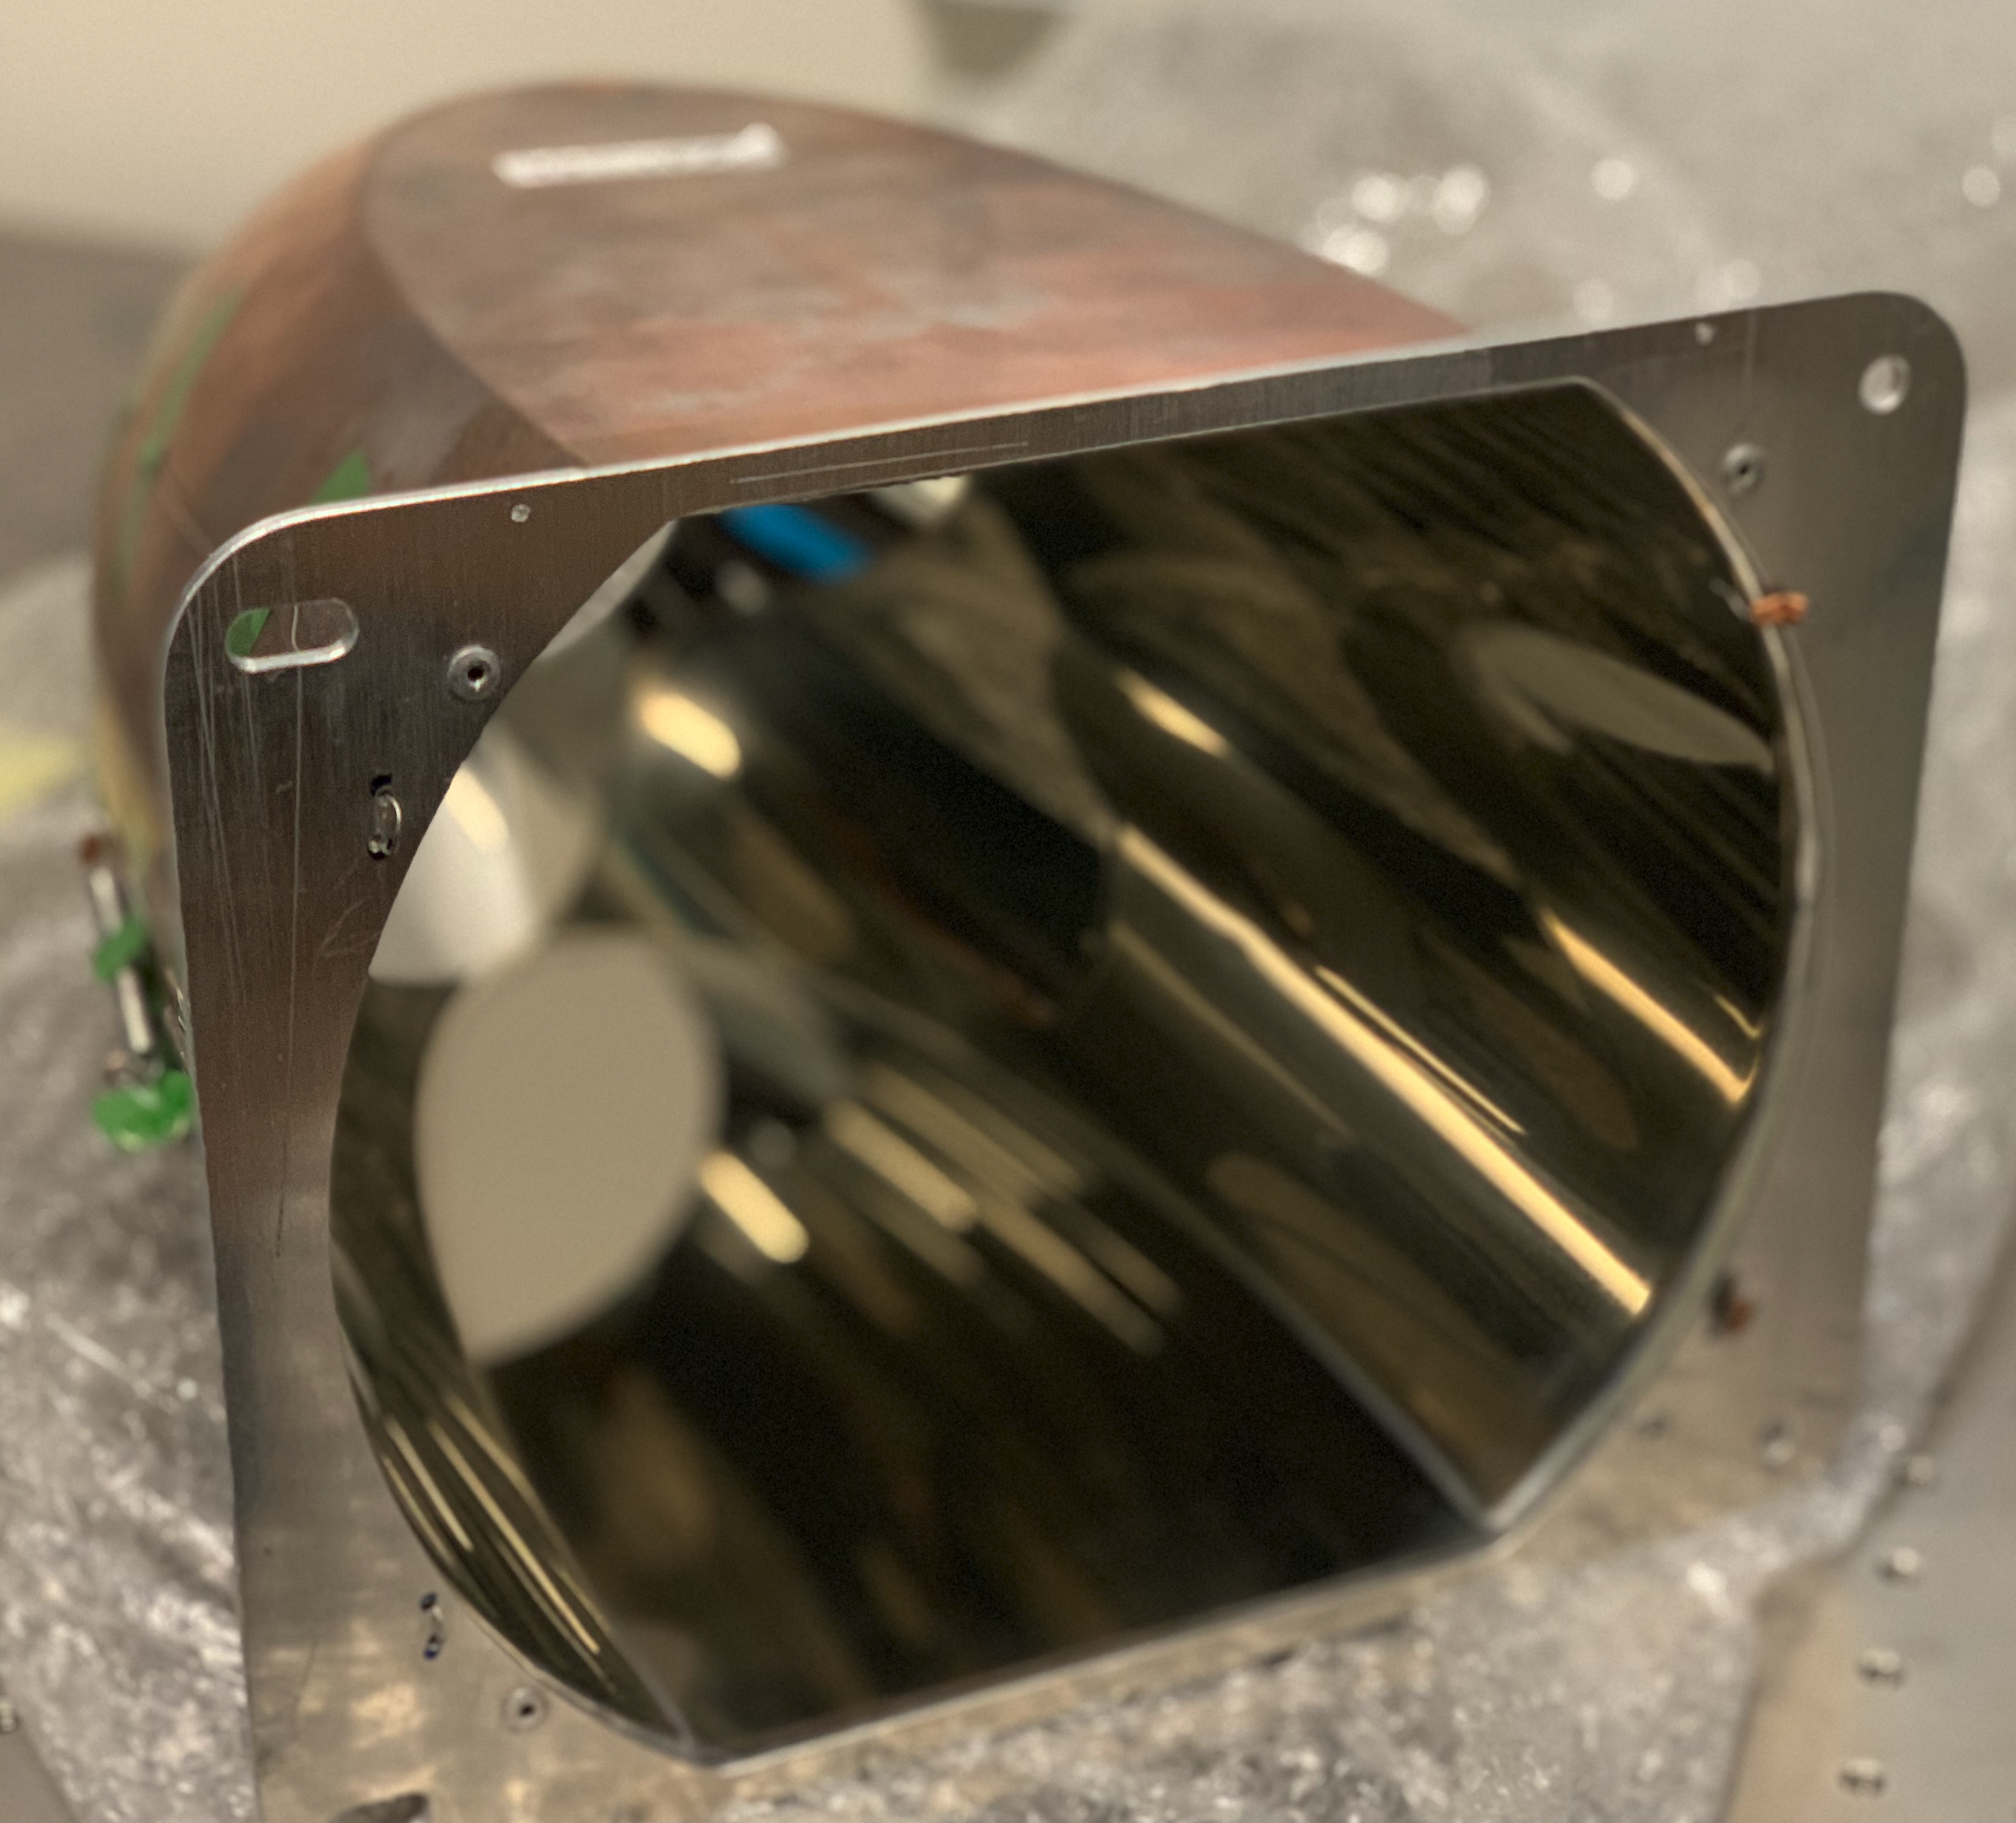
\includegraphics[width=0.99\columnwidth,keepaspectratio]{img/wcLargeReal.png}
	\includegraphics[width=0.99\columnwidth,keepaspectratio]{img/wcLargeSim.png}
	\caption{Top: a photograph of the large WC used for segments 12 to 18. Bottom: the tessellated volume used in the
            simulation, imported from the CAD engineering model.}
	\label{fig:wcSimulation}
\end{figure}

\begin{figure}
	\centering
	\includegraphics[width=0.99\columnwidth,keepaspectratio]{img/simShield.png}
	\caption{The magnetic shields are modeled by mu-metal boxes in the GEMC simulations (black). The WC (grey) focus the light on the red PMT surface.}
	\label{fig:simShield}
\end{figure}


The LTCC box support structure was imported from the engineering model shown in \F{boxCut}. This includes the 1-cm thick aluminum
elliptical and hyperbolic mirror support flanges, the nose, and the hardware mount to the CLAS12 beamline.


\subsection{Digitization}

In the digitization the number of collected photons is converted to charge by taking into account:

\begin{itemize}
	\item The quantum efficiency of the PMTs
	\item The position and width of the single photo-electron peak as stored in the CLAS12 calibration database
\end{itemize}


\subsection{Run Period Variations}

As the start of CLAS12 beam operations, there was not sufficient $C_4F_{10}$ gas to fill all sectors, so some LTCC sectors
where removed from the Forward Carriage. As they were installed or removed, any gas leaks were found and fixed.
These CLAS12 configuration changes are imported in GEMC as database variations of the simulation setup.
The default simulations only include sector 2 (S2), S3, S5, and S6 as the RICH detector replaces the LTCC S1 and S4.
The variations are listed in Table \ref{tab:simVariations}.

\begin{table}
	\begin{center}
		\begin{tabular}{| l | c |}
			\hline \hline
			Run Period       & Sectors Installed and Gas \\
			\hline
			Default          & S2, S3, S5, S6, all $C_4F_{10}$    \\
			RGA Spring 2018  & S2, S3, S6 (N$_2$), S5 ($C_4F_{10}$)  \\
			RGA Fall 2018    & S3 ($C_4F_{10}$), S5 (N$_2$)          \\
			RGB Spring 2018  & S3 ($C_4F_{10}$), S5 ($C_4F_{10}$) \\
			\hline \hline
		\end{tabular}
	\end{center}
	\caption{LTCC simulation variations for different CLAS12 run periods. Shown are which sectors are present and the gas in each sector}
	\label{tab:simVariations}
\end{table}







\section{Performance}

ec performance description


\section{Conclusions}

To address the change of its scope from electron to pion identification for momenta greater than 3.5~GeV,
the original CLAS Cherenkov Counters were refurbished at part of the new CLAS12 Low Threshold Cherenkov
Counter (LTCC) system. The work included improvements of the reflectivities for the mirrors and the Winston
cones, p-terphenyl coating of the PMTs, expansion of the gas volumes, and redesign of the box walls and patch
panels. The LTCC detector sectors after refurbishment are shown in \F{ltccInstalled} installed on the CLAS12
Forward Carriage upstream of the Forward Time-of-Flight system. The average LTCC efficiency for electron
detection in the momentum range from 3.5 to 6.5~GeV is 94\%. The pion efficiency starts around 50\% near
the expected signal threshold, and rises with momentum as expected. A plateau of 88\% is reached at a momentum
of 5~GeV. This is within range of an expectation of efficiency above 90\%. Additional future studies are required
to full quantify the detection efficiency of the CLAS12 LTCC for both positive and negative pions as a function of
momentum.

\begin{figure}
    \centering
    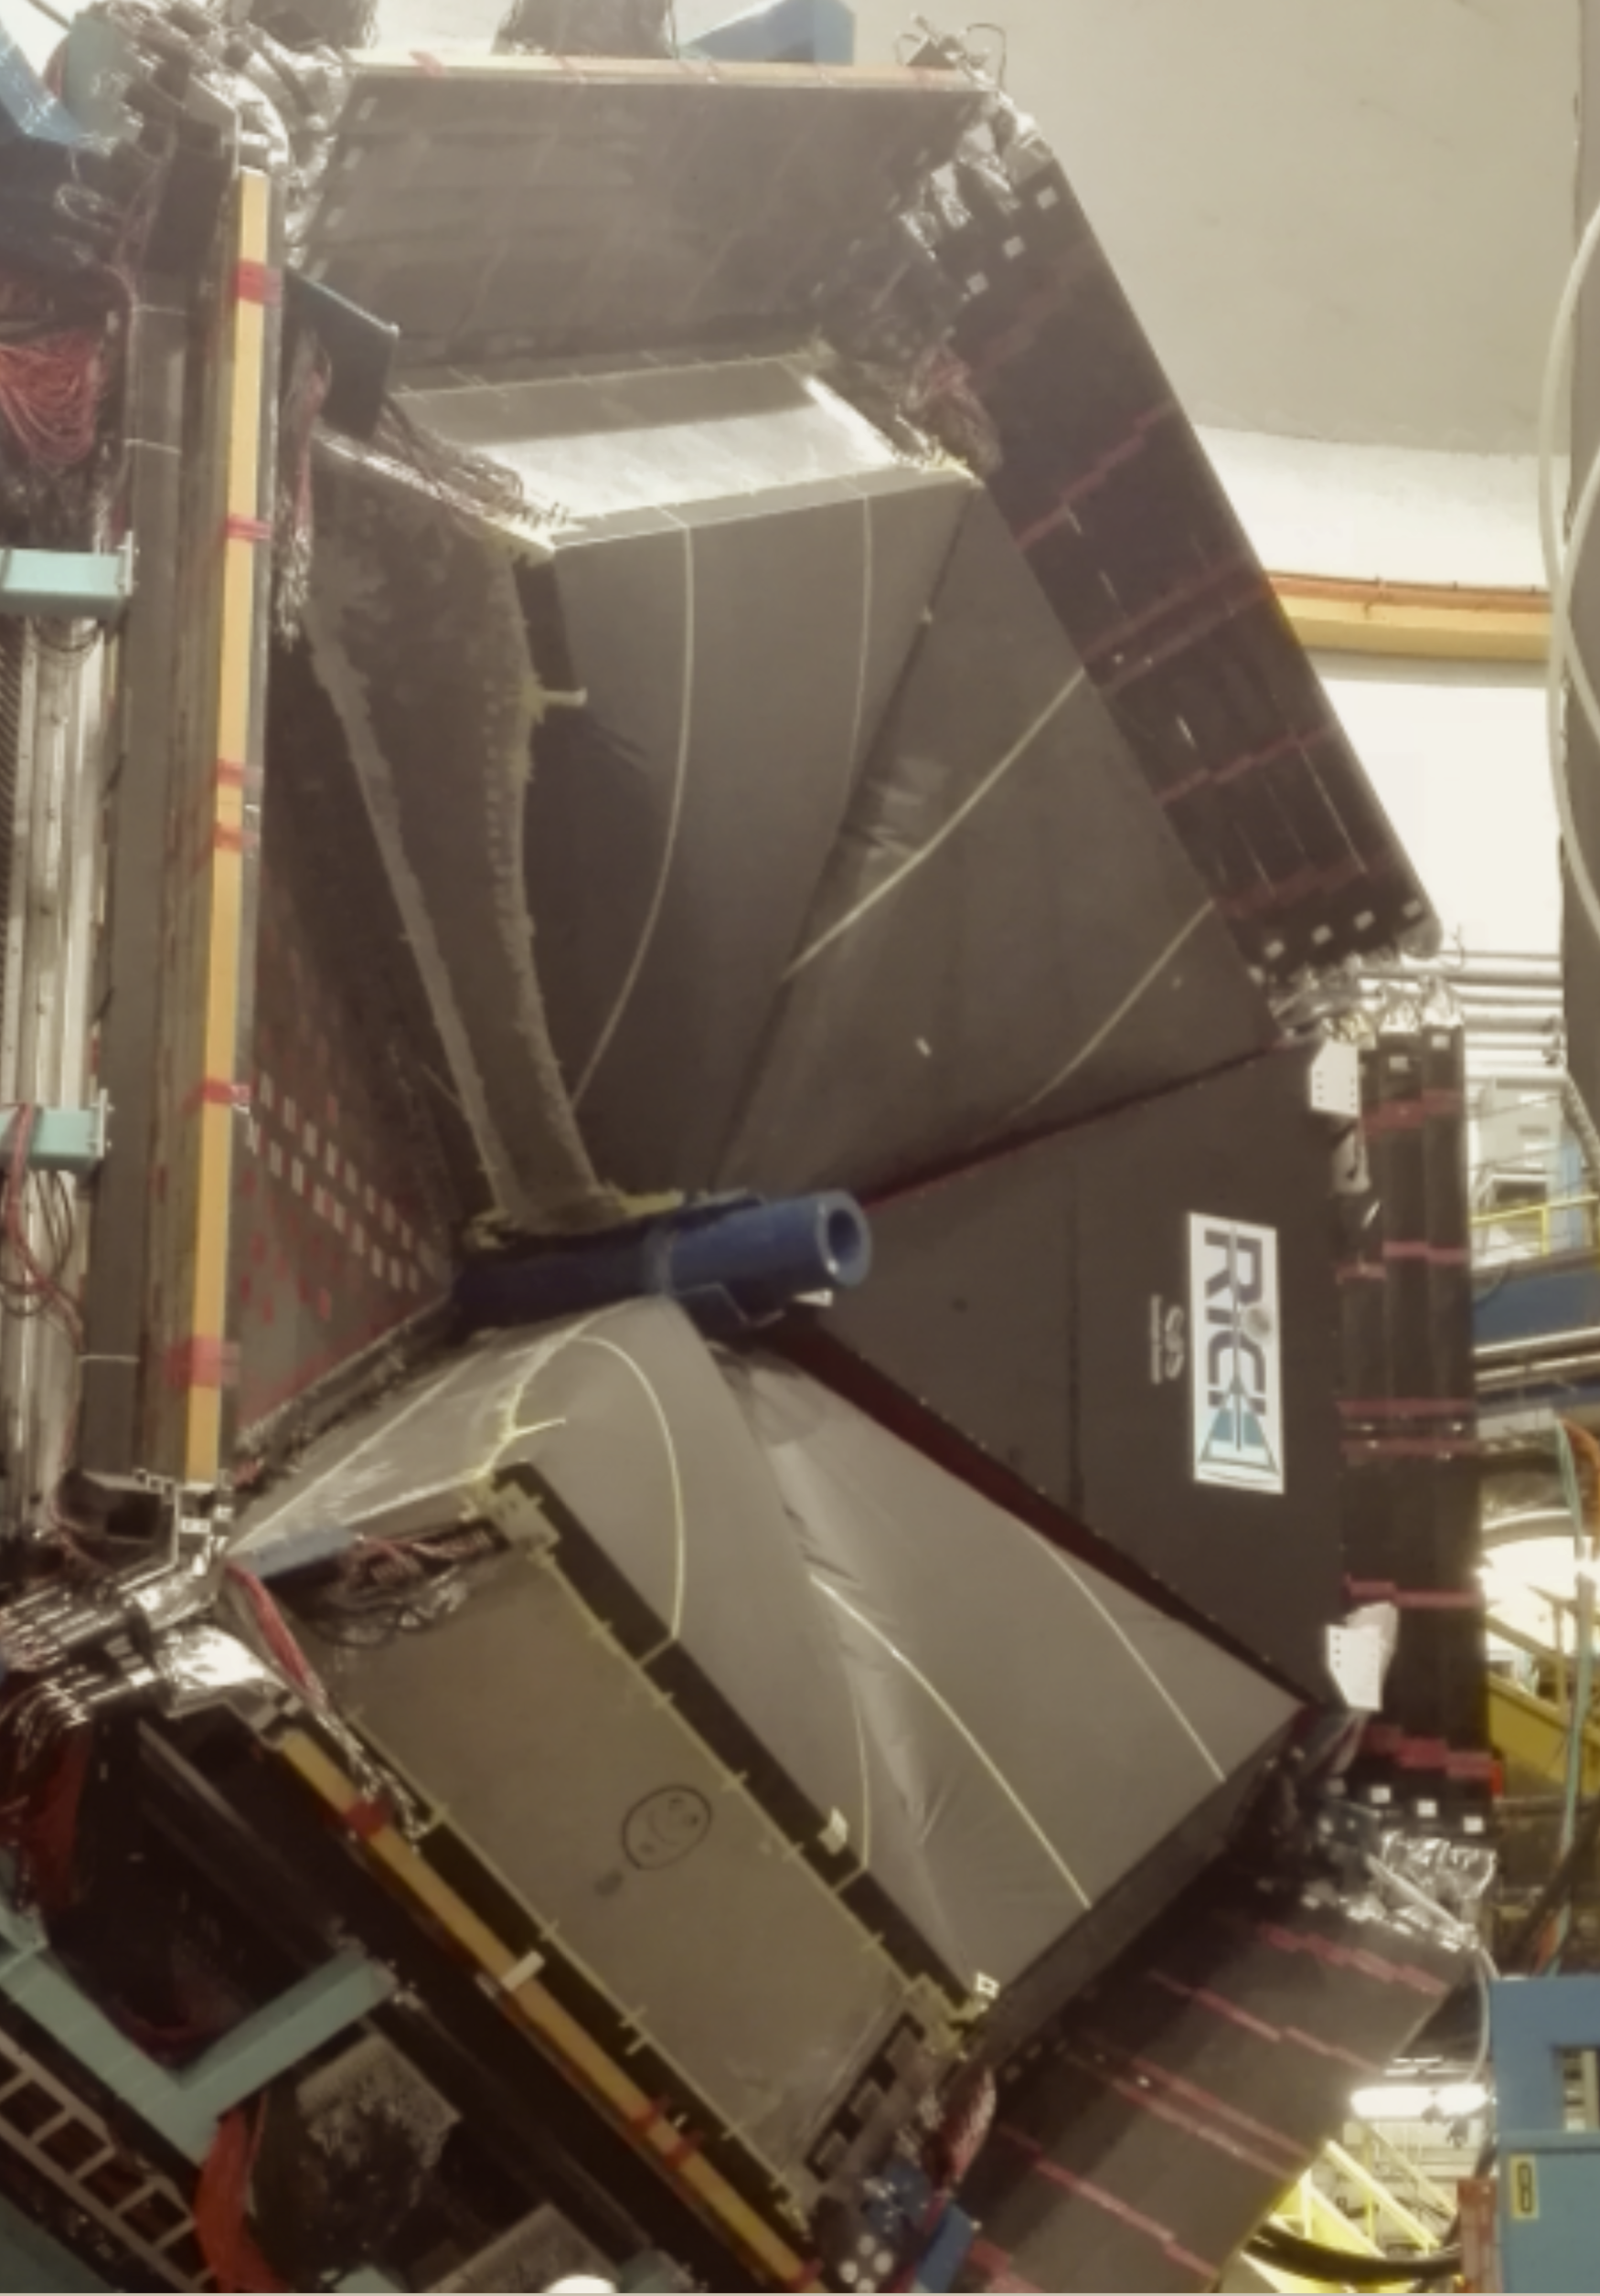
\includegraphics[width=1.0\columnwidth,keepaspectratio]{img/ltccInstalled.png}
    \caption{The LTCC sectors installed after refurbishment on the CLAS12 Forward Carriage. The RICH detector
    is installed in the sector~4 position and the sector~1 position awaits the installation of a second RICH detector.}
    \label{fig:ltccInstalled}
\end{figure}

\section{Acknowledgments}

We thank the Detector Support Group at Jefferson Lab for the work on the cone refurbishment, reflectivity tests,
PMT divider modifications and installation, and for designing the gas control system and associated software. We
thank Temple University for the p-terphenyl deposition. We thank Vladimir Popov for the implementation of the
divider base modification. We thank Youri Sharabian and Steve Christo for their consultations and contributions.
We thank the technical team of Hall~B for their work and dedication on all aspect of the project. Finally, we thank
all the Hall~B staff for their unyielding support. This work was supported in part by
DOE Contract DE-AC05-84ER40150.


\section{References}

\bibliography{bibfile}
\bibliographystyle{elsarticle-num}
\end{document}








